\documentclass{standalone}
\usepackage{tikz}
\begin{document}
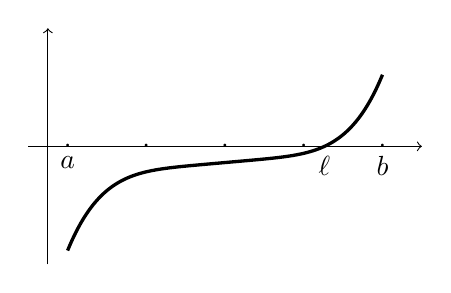
\begin{tikzpicture}%[scale=2,xmin=-2.5,xmax=2.5,ymin=-1.5,ymax=1.5]
%\shorthandoff{:};
%\draw[->] (\xmin,0)--(\xmax,0);
\draw[->] (-2.5,0)--(2.5,0);
%\draw[->] (-2.25,\ymin)--(-2.25,\ymax);
\draw[->] (-2.25,-1.5)--(-2.25,1.5);
%\fenetre
\draw[domain=-2:2, samples=200, very thick]  plot ({\x},{((\x)^5+3*(\x)-7)/34});
\draw (-2,0)node{$\cdot$};
\draw (-1,0)node{$\cdot$};
\draw (1,0)node{$\cdot$};
\draw (0,0)node{$\cdot$};
\draw (2,0)node{$\cdot$};
\draw (-2 , 0) node[below] {$a$};
\draw (2 , 0) node[below] {$b$};
\draw (1.26 , 0) node[below] {$\ell$};
 \end{tikzpicture}
\end{document}

